\documentclass[tikz,border=4pt]{standalone}
\usepackage{ctex}
\usepackage{amsmath}
\usepackage{pgfplots}
\pgfplotsset{compat=1.18}

% p10-01b: |a|大小对比（开口宽窄：y=x^2, y=2x^2, y=0.5x^2）
\begin{document}
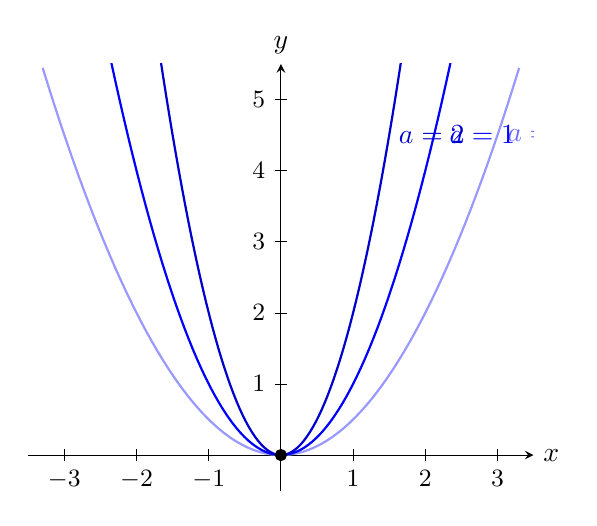
\begin{tikzpicture}
\begin{axis}[
  width=8cm, height=7cm,
  axis lines=center,
  xlabel={$x$}, ylabel={$y$},
  every axis x label/.style={at={(axis cs:3.5,0)}, anchor=west},
  every axis y label/.style={at={(axis cs:0,5.5)}, anchor=south},
  xmin=-3.5, xmax=3.5,
  ymin=-0.5, ymax=5.5,
  xtick={-3,-2,-1,1,2,3},
  ytick={1,2,3,4,5},
  tick style={color=black},
  ticklabel style={font=\small},
  clip=true,
]
  % y = 0.5x^2（a小，开口宽）
  \addplot[blue!40, thick, domain=-3.3:3.3, samples=80] {0.5*x^2};
  \node[right, blue!60] at (axis cs:3.0, 4.5) {$a=\frac{1}{2}$};

  % y = x^2（a=1）
  \addplot[blue, thick, domain=-2.35:2.35, samples=80] {x^2};
  \node[right, blue] at (axis cs:2.2, 4.5) {$a=1$};

  % y = 2x^2（a大，开口窄）
  \addplot[blue!80!black, thick, domain=-1.67:1.67, samples=80] {2*x^2};
  \node[right, blue!80!black] at (axis cs:1.5, 4.5) {$a=2$};

  % 原点
  \addplot[only marks, mark=*, mark size=2pt] coordinates {(0,0)};
\end{axis}
\end{tikzpicture}
\end{document}
